% Model report generated by SolverMapp.
% Compile with: pdflatex, bibtex, pdflatex, pdflatex (references.bib is written by the first run).
\begin{filecontents*}[overwrite]{references.bib}
@misc{ref,
  note   = {First-order reaction network},
  key    = {First-order reaction network}
}
\end{filecontents*}
\documentclass[11pt,a4paper]{article}
\usepackage[T1]{fontenc}
\usepackage[utf8]{inputenc}
\usepackage{lmodern}
\usepackage{amsmath,amssymb}
\usepackage{booktabs,longtable}
\usepackage{siunitx}
\usepackage{algorithm}
\usepackage{algpseudocode}
\usepackage{tikz}
\usetikzlibrary{positioning,shapes.geometric,shapes.misc,arrows.meta}
\usepackage{adjustbox}
\usepackage[hidelinks]{hyperref}

\title{Linear species network in index notation}
\author{}
\date{\today}

\begin{document}
\maketitle

The model consists of 2 equations in 5 variables: 3 inputs, 1 state variable, 0 intermediate variables and 1 output. It is solved in 2 steps (Algorithm~\ref{alg:solution}).

\section{Nomenclature}
\begin{longtable}{@{}l p{0.48\linewidth} l l@{}}
  \toprule
  Symbol & Description & Unit & Value \\
  \midrule
  \endhead
  \bottomrule
  \endfoot
  \multicolumn{4}{@{}l}{\textit{Inputs}} \\
  $K$ & Rate matrix (columns sum to 0) & \si{1/s} & -2, 0, 0; 1.5, -1, 0.5; 0.5, 1, -0.5 \\
  $t$ & Time & \si{s} & \num{0} \\
  $M$ & Number of species & -- & \num{3} \\
  \addlinespace
  \multicolumn{4}{@{}l}{\textit{State variables}} \\
  $c$ & Concentrations & \si{mol/m^{3}} & 1, 0, 0 \\
  \addlinespace
  \multicolumn{4}{@{}l}{\textit{Outputs}} \\
  $c_{tot}$ & Total concentration & \si{mol/m^{3}} &  \\
\end{longtable}

\section{Governing equations}

\subsection{Species balance}
Source: \cite{ref}, Eq.~(1).
\begin{equation}
  \frac{dc_i}{dt} = \sum_j K_{ij} c_j
  \label{eq:species-balance}
\end{equation}
\noindent where

\noindent\begin{tabular}{@{\quad}l@{\quad}p{0.7\linewidth}@{}}
  $c$ & Concentrations, \si{mol/m^{3}} \\
  $K$ & Rate matrix (columns sum to 0), \si{1/s} \\
  $t$ & Time, \si{s} \\
\end{tabular}

\noindent Holds for every $i = 1, \dots, M$. Integrated over $t$ from $0$ to $2$ with the classical fourth-order Runge–Kutta method in 200 steps, starting from the start value of $c$.

\subsection{Total}
Source: \cite{ref}, Eq.~(2).
\begin{equation}
  c_{tot} = \sum_i c_i
  \label{eq:total}
\end{equation}
\noindent where

\noindent\begin{tabular}{@{\quad}l@{\quad}p{0.7\linewidth}@{}}
  $c_{tot}$ & Total concentration, \si{mol/m^{3}} \\
  $c$ & Concentrations, \si{mol/m^{3}} \\
\end{tabular}


\section{Solution algorithm}
\begin{algorithm}[htbp]
  \caption{Solution procedure}\label{alg:solution}
  \begin{algorithmic}[1]
    \State Set the inputs $K$ and $M$
    \State Set the start values $c$
    \For{$t = 0$ to $2$ in 200 steps} \Comment{RK4}
      \State Advance $c$ by one RK4 step of Eq.~\eqref{eq:species-balance}
    \EndFor
    \State Compute $c_{tot}$ from Eq.~\eqref{eq:total}
  \end{algorithmic}
\end{algorithm}

Figure~\ref{fig:flowchart} shows the same procedure as a flowchart.

\begin{figure}[htbp]
  \centering
  \begin{adjustbox}{max width=\linewidth, max totalheight=0.9\textheight}
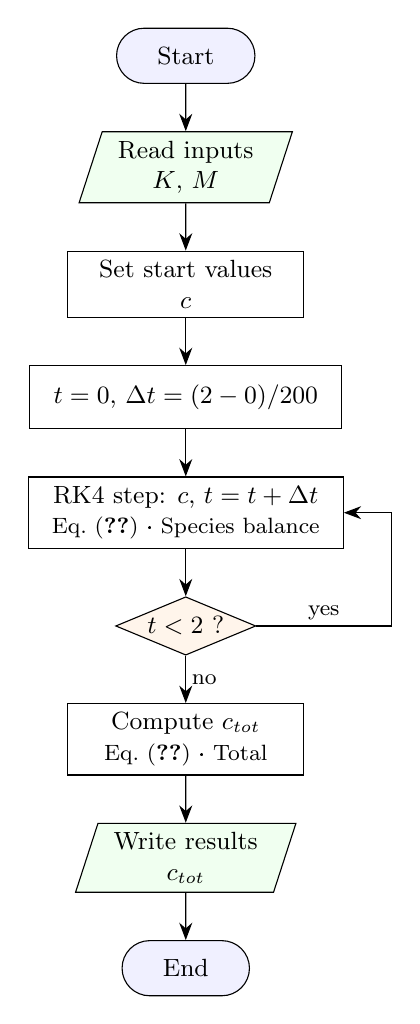
\begin{tikzpicture}[
  node distance=6mm, >={Stealth[length=2.2mm]}, font=\small,
  every node/.style={align=center},
  term/.style={draw, rounded rectangle, minimum height=7mm, inner xsep=5mm, fill=blue!6},
  io/.style={draw, trapezium, trapezium left angle=72, trapezium right angle=108, trapezium stretches body, minimum height=8mm, inner xsep=2mm, fill=green!6},
  proc/.style={draw, rectangle, minimum height=8mm, minimum width=30mm, inner xsep=3mm},
  dec/.style={draw, diamond, aspect=2.4, inner sep=1pt, fill=orange!8},
  lbl/.style={font=\footnotesize, inner sep=2pt}]
  \node[term] (n1) {Start};
  \node[io, below=of n1] (n2) {Read inputs \\ $K$, $M$};
  \node[proc, below=of n2] (n3) {Set start values \\ $c$};
  \node[proc, below=of n3] (n4) {$t = 0$, $\Delta t = (2 - 0) / 200$};
  \node[proc, below=of n4] (n5) {RK4 step: $c$, $t = t + \Delta t$ \\ {\footnotesize Eq.~\eqref{eq:species-balance} \textperiodcentered{} Species balance}};
  \node[dec, below=of n5] (n6) {$t < 2$ ?};
  \node[proc, below=of n6] (n7) {Compute $c_{tot}$ \\ {\footnotesize Eq.~\eqref{eq:total} \textperiodcentered{} Total}};
  \node[io, below=of n7] (n8) {Write results \\ $c_{tot}$};
  \node[term, below=of n8] (n9) {End};
  \coordinate (E) at (current bounding box.east);
  \coordinate (L0) at ([xshift=6mm]E);
  \draw[->] (n1) -- (n2);
  \draw[->] (n2) -- (n3);
  \draw[->] (n3) -- (n4);
  \draw[->] (n4) -- (n5);
  \draw[->] (n5) -- (n6);
  \draw[->] (n6) -- node[lbl, right] {no} (n7);
  \draw[->] (n7) -- (n8);
  \draw[->] (n8) -- (n9);
  \draw[->] (n6.east) -- node[lbl, above] {yes} (n6.east -| L0) |- (n5.east);
\end{tikzpicture}
  \end{adjustbox}
  \caption{Flowchart of the solution procedure}\label{fig:flowchart}
\end{figure}

\bibliographystyle{plain}
\bibliography{references}

\end{document}